
\begin{frame}{‌الگوریتم فلوید-وارشال}
\begin{itemize}\itemr
\item[-]
الگوریتم فلوید-وارشال
\fn{1}{Floyed-Warshall algorithm}
مسئله کوتاهترین مسیر بین همهٔ جفت‌ها را در زمان
\m{O(V^3)}
حل می‌کند. در این الگوریتم یال‌ها با وزن منفی می‌توانند وجود داشته باشند، اما دورها با وزن منفی در گراف ورودی مسئله مجاز نیستند.
این الگوریتم یک الگوریتم از نوع برنامه‌ریزی پویا است.
\end{itemize}
\end{frame}


\begin{frame}{‌الگوریتم فلوید-وارشال}
\begin{itemize}\itemr
\item[-]
رئوس گراف
\m{G}
را با اعداد صحیح شماره گذاری می‌کنیم. بنابراین خواهیم داشت
\m{V = \{1,2, \cdots, n\}} .
\item[-]
برای حل این مسئله با استفاده از برنامه‌ریزی پویا ابتدا کوتاهترین مسیر بین رئوس 
\m{i}
و
\m{j}
را با فرض اینکه
هیچ رأسی در مسیر وجود نداشته باشد محاسبه می‌کنیم. در صورتی که یال
\m{(i,j)}
وجود داشته باشد، طول چنین مسیری برابر با وزن این یال است.
سپس کوتاهترین مسیر بین رئوس
\m{i}
و
\m{j}
را با فرض بر اینکه
 فقط رأس 
\m{1}
در مسیر
 وجود داشته باشد به دست می‌آوریم. سپس فرض می‌کنیم رأس 
\m{2}
  نیز وجود داشته باشد
و کوتاهترین مسیر بین همهٔ جفت رئوس را با فرض اینکه رئوس میانی مسیر
در مجموعهٔ
\m{\{1, 2 \}}
باشند محاسبه می‌کنیم.
\item[-]
 به همین ترتیب 
به ازای
\m{1 \leqslant k \leqslant n}
زیر مجموعهٔ
\m{\{1,2, \cdots, k\}}
از رئوس را در نظر می‌گیریم و به ازای هر جفت از رئوس
\m{i,j \in V}
، همه مسیرها از
\m{i}
به
\m{j}
را که از رئوس
\m{\{1,2, \cdots, k\}}
می‌گذرند را در نظر می‌گیریم و فرض می‌کنیم
\m{p}
کوتاهترین مسیر بین همهٔ این مسیرها باشد.
\end{itemize}
\end{frame}


\begin{frame}{‌الگوریتم فلوید-وارشال}
\begin{itemize}\itemr
\item[-]
حال حالت‌های زیر را در نظر می‌گیریم.
\item[-]
اگر
\m{k}
یک رأس میانی در مسیر
\m{p}
نباشد، آنگاه همهٔ رئوس میانی مسیر
\m{p}
متعلق به مجموعهٔ
\m{\{1,2, \cdots, k-1\}}
هستند. بنابراین کوتاهترین مسیر از رأس
\m{i}
به رأس
\m{j}
با رئوس میانی
\m{\{1,2, \cdots, k\}} ,
همان
کوتاهترین مسیر از
\m{i}
به
\m{j}
با رئوس میانی در مجموعهٔ
\m{\{1,2, \cdots, k-1\}}
است.
\item[-]
اگر
\m{k}
یک رأس میانی در مسیر
\m{p}
باشد، آنگاه مسیر
\m{p}
را به دو قسمت
\m{i \stackrel{p_1}{\leadsto} k \stackrel{p_2}{\leadsto}j }
تقسیم می‌کنیم. 
 چون رأس
\m{k}
یک رأس میانی در مسیر
\m{p_1}
نیست، همهٔ رئوس میانی در مسیر
\m{p_1}
به مجموعهٔ
\m{\{1,2, \cdots, k-1\}}
تعلق دارند. بنابراین
\m{p_1}
کوتاهترین مسیر از
\m{i}
به
\m{k}
با همهٔ رئوس میانی
\m{\{1,2, \cdots, k-1\}}
است. همچنین
\m{p_2}
کوتاهترین مسیر از رأس
\m{k}
به رأس
\m{j}
با همهٔ رئوس میانی در مجموعهٔ
\m{\{1,2, \cdots, k-1\}}
است.
\end{itemize}
\end{frame}


\begin{frame}{‌الگوریتم فلوید-وارشال}
\begin{itemize}\itemr
\item[-]
شکل زیر این تقسیم بندی مسیر را نشان می‌دهد.
\begin{figure}
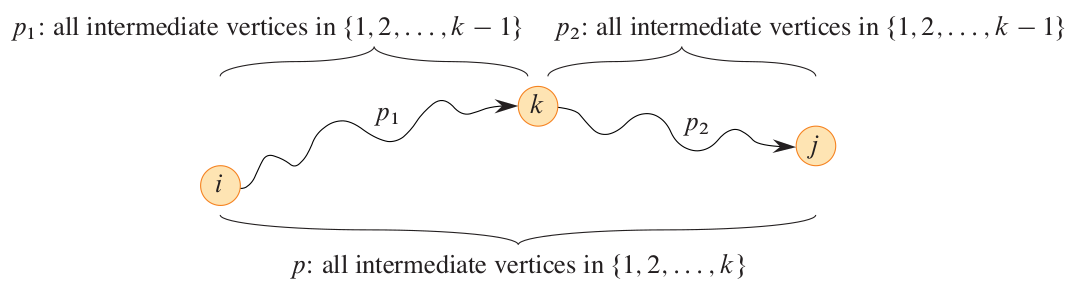
\includegraphics[width=0.9\textwidth]{figs/chap07/656-floyd}
\end{figure}
\end{itemize}
\end{frame}


\begin{frame}{‌الگوریتم فلوید-وارشال}
\begin{itemize}\itemr
\item[-]
بر اساس مشاهدهٔ قبلی می‌توانیم جواب مسئله کوتاهترین مسیر بین جفت‌ها را به صورت یک رابطهٔ بازگشتی بیان کنیم.
\item[-]
فرض کنید
\m{d_{ij}^{(k)}}
طول کوتاهترین مسیر از
\m{i}
به
\m{j}
باشد به طوری‌که رئوس میانی متعلق به مجموعه
\m{\{1,2, \cdots, k\}}
باشند.
\end{itemize}
\end{frame}


\begin{frame}{‌الگوریتم فلوید-وارشال}
\begin{itemize}\itemr
\item[-]
وقتی
\m{k = 0}
است، یک مسیر از رأس
\m{i}
به رأس
\m{j}
که هیچ رأس میانی با شماره‌ای بزرگ‌تر از
\m{0}
نداشته باشد، درواقع هیچ رأس میانی ندارد. چنین مسیری حداکثر یک یال دارد، بنابراین
\m{d_{ij}^{(0)} = w_{ij}}
\item[-]
می‌توانیم مقدار
\m{d_{ij}^{(k)}}
را به صورت بازگشتی تعریف کنیم.
\begin{align*}
\m{d_{ij}^{(k)}} = \left\{\begin{array}{lr}
          \m{w_{ij}}& \m{k = 0}~\text{اگر}\\
          \m{min\{d_{ij}^{(k-1)} , d_{ik}^{(k-1)} + d_{kj}^{(k-1)} \}}& \m{k \geqslant 1}~\text{اگر}
\end{array}\right.
\end{align*}
\item[-]
چون برای هر مسیر، همهٔ رئوس میانی متعلق به مجموعهٔ
\m{\{1,2, \cdots, k\}}
هستند، بنابراین ماتریس
\m{D^n = (d_{ij}^{(n)})}
شامل جواب پایانی است. به ازای هر
\m{i,j \in V}
داریم
\m{d_{ij}^{(n)} = \delta(i,j)} .
\end{itemize}
\end{frame}


\begin{frame}{‌الگوریتم فلوید-وارشال}
\begin{itemize}\itemr
\item[-]
الگوریتم فلوید-وارشال از رابطه بازگشتی محاسبه شده استفاده می‌کند و توسط یک روند پایین به بالا مقدار بالا
\m{d_{ij}^{(k)}}
را به ازای
\m{k}
های متفاوت از کوچک به بزرگ محاسبه می‌کند.
\end{itemize}
\end{frame}


\begin{frame}{‌الگوریتم فلوید-وارشال}
\begin{itemize}\itemr
\item[-]
گراف زیر را در نظر بگیرید.
\begin{figure}
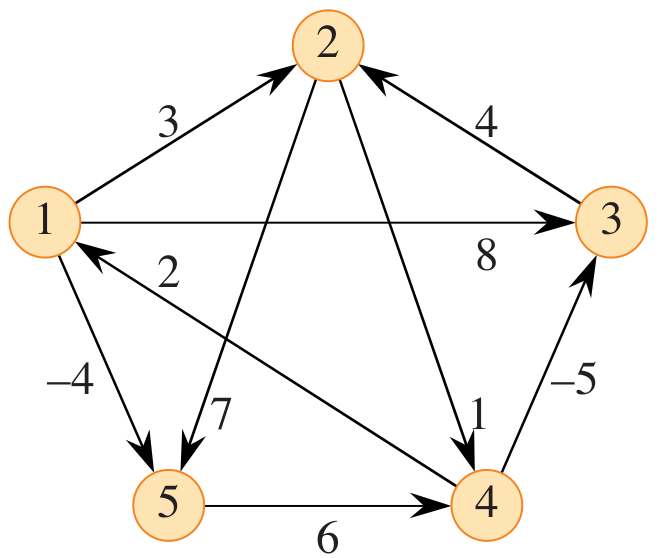
\includegraphics[width=0.4\textwidth]{figs/chap07/652-graph}
\end{figure}
\end{itemize}
\end{frame}

\begin{frame}{‌الگوریتم فلوید-وارشال}
\begin{itemize}\itemr
\item[-]
شکل زیر فرایند محاسبه ماتریس‌های
\m{D^{(k)}}
و
\m{\Pi^{(k)}}
را برای این گراف نشان می‌دهد.
\begin{figure}
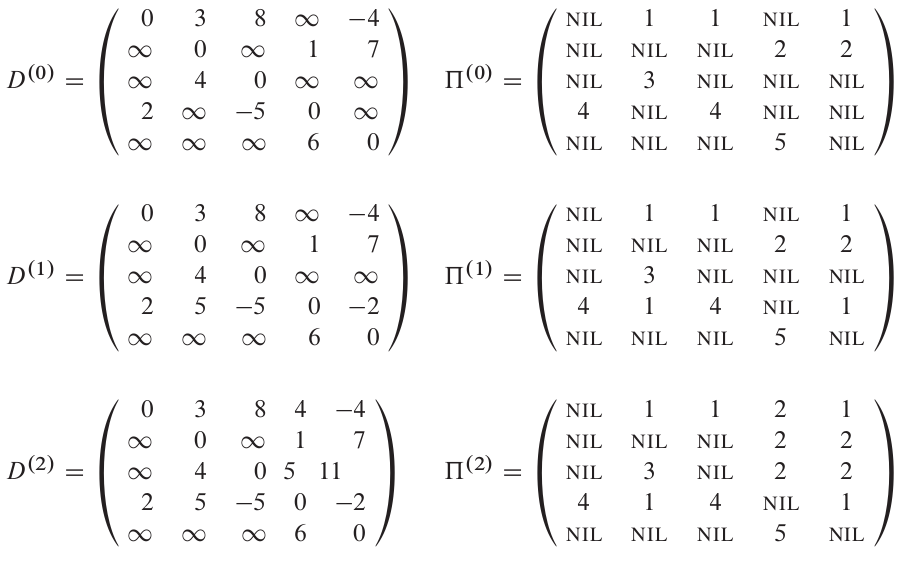
\includegraphics[width=0.6\textwidth]{figs/chap07/658-floyd-pi-1}
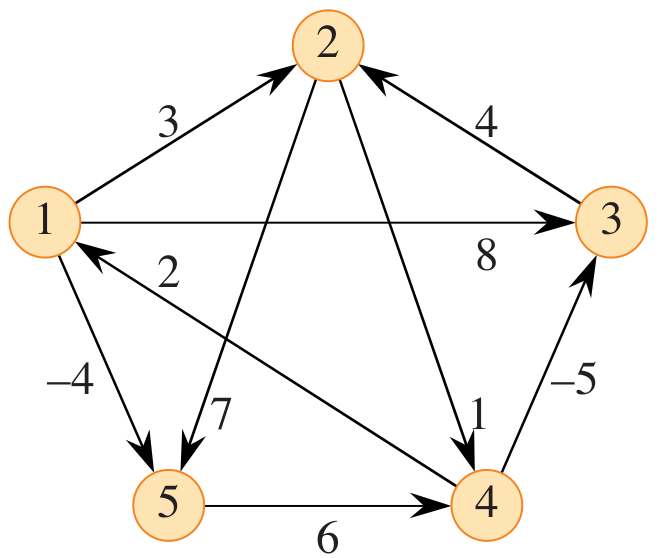
\includegraphics[width=0.3\textwidth]{figs/chap07/652-graph}
\end{figure}
\end{itemize}
\end{frame}


\begin{frame}{‌الگوریتم فلوید-وارشال}
\begin{itemize}\itemr
\item[-]
شکل زیر فرایند محاسبه ماتریس‌های
\m{D^{(k)}}
و
\m{\Pi^{(k)}}
را برای این گراف نشان می‌دهد.
\begin{figure}
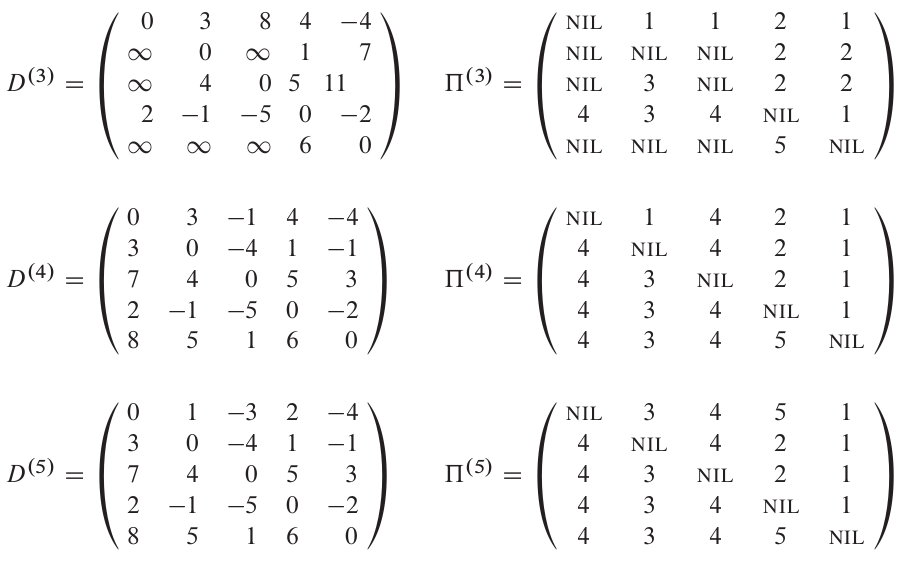
\includegraphics[width=0.6\textwidth]{figs/chap07/658-floyd-pi-2}
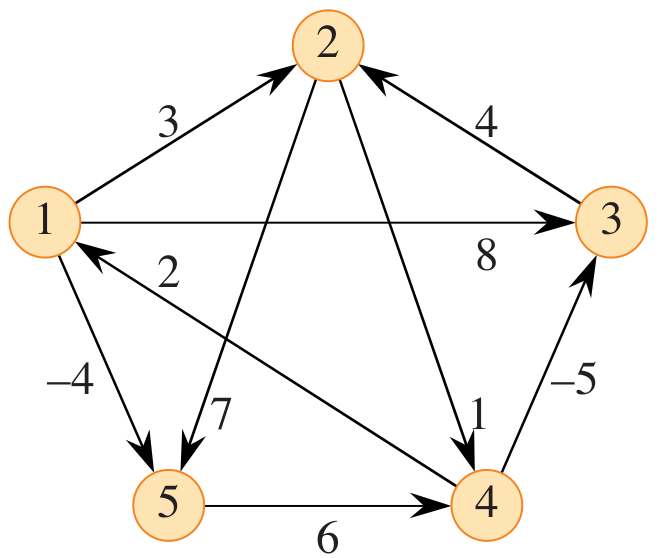
\includegraphics[width=0.3\textwidth]{figs/chap07/652-graph}
\end{figure}
\end{itemize}
\end{frame}



\begin{frame}{‌الگوریتم فلوید-وارشال}
\begin{itemize}\itemr
\item[-]
الگوریتم فلوید-وارشال به صورت زیر است.
\begin{algorithm}[H]\alglr
  \caption{Floyd-Warshall} 
  \begin{algorithmic}[1]
   \Func{Floyd-Warshall}{W,n}
   \State \mc{D^{(0)}} = W
   \For{k = 1 \To n}
   		\State let \mc{D^{(k)}} = (\mc{d_{ij}^{(k)}}) be a new n \mc{\times} n matrix
   		\For{i = 1 \To n}
   				\For{j = 1 \To n}
   						\State \mc{d_{ij}^{(k)}} = \mc{\min \{d_{ij}^{(k-1)} , d_{ik}^{(k-1)} + d_{kj}^{(k-1)}\}}
   				\EndFor
   		\EndFor
   	\EndFor
   	\State \Return \mc{D^{(n)}}                       
  \end{algorithmic}
  \label{alg:merge}
\end{algorithm}
\end{itemize}
\end{frame}


\begin{frame}{‌الگوریتم فلوید-وارشال}
\begin{itemize}\itemr
\item[-]
در الگوریتم فلوید-وارشال سه حلقه
\code{for}
تودرتو وجود دارد. چون محاسبه خط ۶ برنامه در زمان
\m{O(1)}
انجام می‌شود، بنابراین این الگوریتم در زمان
\ath{n^3}
محاسبه می‌شود.
\end{itemize}
\end{frame}


\begin{frame}{‌الگوریتم فلوید-وارشال}
\begin{itemize}\itemr
\item[-]
ماتریس رئوس ماقبل
\m{\Pi}
نیز می‌تواند در زمان محاسبهٔ
\m{D^{(0)}}
،
\m{D^{(1)}}
،
\m{\cdots}
،
\m{D^{(n)}}
محاسبه شود.
\item[-]
به عبارت دیگر می‌توانیم
\m{\Pi^{0}}
،
\m{\Pi^{1}}
،
\m{\cdots}
،
\m{\Pi^{n}}
را محاسبه کنیم به طوری‌که
\m{\Pi = \Pi^{(n)}}
و
\m{\pi_{ij}^{(k)}}
رأس ماقبل رأس
\m{j}
در کوتاهترین مسیری است که از رأس
\m{i}
شروع می‌شود و همهٔ رئوس میانی در مجموعه
\m{\{1,2, \cdots, k\}}
را شامل می‌شود.
\item[-]
مقدار
\m{\pi_{ij}^{(k)}}
را می‌توانیم به صورت بازگشتی تعریف کنیم.
\item[-]
وقتی
\m{k = 0}
است، کوتاهترین مسیر از
\m{i}
به
\m{j}
هیچ رأس میانی ندارد، بنابراین داریم :
\begin{align*}
\m{\pi_{ij}^{(0)}} = \left\{\begin{array}{lrr}
          \text{NIL}& \m{w_{ij}=\infty}~\text{یا} & \m{i = j}~\text{اگر}\\
          \m{i}& \m{w_{ij} < \infty}~\text{و} & \m{i \neq j}~\text{اگر}\\
\end{array}\right.
\end{align*}
\end{itemize}
\end{frame}


\begin{frame}{‌الگوریتم فلوید-وارشال}
\begin{itemize}\itemr
\item[-]
به ازای
\m{k \geqslant 1}
، اگر کوتاهترین مسیر از رأس 
\m{i}
به
\m{j}
، رأس
\m{k}
را به عنوان رأس میانی شامل نشود، 
آنگاه رأس ماقبل 
\m{j}
در مسیری که
 با رئوس میانی
\m{\{1,2, \cdots, k\}}
 از 
\m{i}
آغاز شده است
برابر است با رأس ماقبل
\m{j}
در مسیری که 
 با رئوس میانی
\m{\{1,2, \cdots, k-1\}}
از 
\m{i}
آغاز شده است.
\item[-]
اگر کوتاهترین مسیر از رأس 
\m{i}
به
\m{j}
، رأس
\m{k}
را به عنوان رأس میانی شامل شود،
به طوری که
\m{i {\leadsto} k {\leadsto}j }
و
\m{k \neq j}
، آنگاه رأس ماقبل رأس
\m{j}
در این مسیر همان رأس ماقبل
\m{j}
در مسیری است که از
\m{k}
آغاز می‌شود و شامل همهٔ رئوس در مجموعهٔ
\m{\{1,2, \cdots, k-1\}}
می‌شود.
\item[-]
پس به ازای
\m{k \geqslant 1}
داریم :
\begin{align*}
\m{\pi_{ij}^{(k)}} = \left\{\begin{array}{lr}
          \m{\pi_{kj}^{(k-1)}}& \m{d_{ij}^{(k-1)} > d_{ik}^{(k-1)} + d_{kj}^{(k-1)}}~\text{اگر}\\
          \m{\pi_{ij}^{(k-1)}}& \m{d_{ij}^{(k-1)} \leqslant d_{ik}^{(k-1)} + d_{kj}^{(k-1)}}~\text{اگر}
\end{array}\right.
\end{align*}
\end{itemize}
\end{frame}
